\chapter{Circuit Evaluation with Active Security}
\label{cha:CEPS}

asdasd

\iffalse
\emph{Proof-of-Stake} (PoS) \cite{pos} is an alternative approach to obtain consensus for public blockchains, compared to \emph{Proof-of-Work}. Instead of having miners that are rewarded by solving cryptographic puzzles, a set of validators, also known as stakeholders, take turns proposing or voting on the next block. How much of a say a validator has, depends on the amount of the currency he has, also known as \emph{stake}. The advantage of this is that wasteful hashing is no longer needed, which has high energy consumption as explained previously in section \ref{subsec:anal-bitcoin}. It also incentivizes the stakeholders to maintain the integrity of the chain, as the value of the content on the blockchain diminishes the stakeholders will suffer the biggest impact.\\

As these types of protocols do not rely on Proof-of-Work, i.e., wasteful hashing, they use a lot less electricity. Creating attacks such as $>50\%$ will be very expensive as you are betting your fortune to attack the chain and it gives the possibility to use game-theoretic design to discourage centralized cartels, and acting harmfully against the network.\\

There are two major types of PoS \cite{eth-pos}
\begin{enumerate}
    \item The \textbf{chain-based PoS} selects a validator to create a new block within some fixed period. The created block must reference a block previously on the blockchain, usually the last block on the longest chain.
    
    \item The \textbf{Byzantine fault tolerance-style PoS} allows validators to propose blocks, but agreeing on which blocks to use is done through a voting system. At the end, all validators agree on which blocks are part of the chain and which are not.
\end{enumerate}

Proof-of-Stake type consensus protocols are not necessarily bound to the stake a user has but can use alternative systems that instead could rely on electing stakeholder. An example of this is the cryptocurrency \emph{NEO} \cite{neo}, which uses a variation in which, all users who hold the NEO currency can vote for representatives called bookkeepers. In which the representatives have public identities and operate something closely resembling the Byzantine fault tolerance-style PoS. The NEO-system resembles how governments elect representatives to make decisions.\\

For analyzing Proof-of-Stake, this thesis will focus on two implementations of PoS consensus, namely \emph{Ouroboros} and \emph{Ouroboros: Praos}. These protocols were selected due to the emphasis on showing a provably correct protocol and have been accepted as papers to conferences from the International Association for Cryptologic Research \cite{iacr-ouro}\cite{iacr-praos}. Both of the papers are relatively new from August and November 2017, respectively. Despite the recent release of the papers, they obtain credibility by being peer reviewed at conferences, where they were presented to peers within the science of cryptology. Both of these protocols use the chain-based PoS approach in which leaders are selected based on their stake to create new blocks. It should be noted that these protocols also contain co-authors from the Bitcoin Backbone protocol \cite{bitcoin-backbone}, which was used for the analysis of Bitcoin. As a result of this many of the approaches for showing security having common characteristics.

Both of these protocols will first be given a design section where the protocol loosely will be explained intuitively. The design section will be the followed by a formal analysis of the protocol and models used to show security. At the end of both protocols, a joint discussion will be presented to compare the general structure of their protocol, as well as comparing the security.


% Ouroboros
\section{Ouroboros}
One implementation of a PoS protocol is Ouroboros \cite{ouroboros}. Ouroboros shares a common author with the analysis done in the Bitcoin backbone protocol. This is heavily reflected in the analysis of Ouroboros proving the same properties for it to be a secure blockchain protocol and using resembling models for the protocol. Additionally it was included in the 37th Annual International Cryptology Conference, which exposes it even further to its peers for peer review and further analysis.

For the overview of the Ouroboros protocol the design will first be covered followed by a formal analysis showing the three properties also showed in the Bitcoin backbone protocol; \emph{chain growth}, \emph{chain quality} and \emph{common prefix}.


\subsection{Design}
% slots
For the model used in Ouroboros the time is split into discrete units called \emph{slots}. These slots can potentially contain a single block on the blockchain. Each player within the system is equipped with roughly synchronized clocks that indicate the current slot. This allows them to carry out a distributed protocol intending to collectively assign a block to this current slot. Each slot is indexed by an incrementing integer, $sl_r \; | \; r \in \{1,2,\dots \}$. \\

% blocks
The first block created on the chain is called the genesis block. This block contains the list of stakeholders, who are identified by their public-keys $vk$, their stakes and some auxiliary information $\rho$, which is used to seed the slot leader election process. The slot leader election process determines which stakeholder is allowed to propose a block at a given slot. This process is defined as follows in \cite{ouroboros}.

% leaders and leaderselection
\begin{mydef}[Leader Selection Process]
\label{def:ouro-leader}
A leader selection process with respect to stakeholder distribution $\mathbb{S} = \{(vk_1, s_1), \ldots, (vk_n, s_n)\}$, $(D,F)$ is a pair consisting of a distribution and a deterministic function such that, when $\rho \xleftarrow{} D$ it holds that for all $sl_j \in \{sl_1, \ldots sl_R\}$, $F(\mathbb{S},\rho,sl_j)$ outputs $U_i \in \{U_1,\ldots, U_n\}$ with probability
\begin{equation*}
    p_i = \frac{s_i}{\sum_{k=1}^n s_k},
\end{equation*}
where $s_i$ is the stake held by stakeholder $U_i$. Furthermore, the family of random variables $\{ F(\mathbb{S}, \rho, sl_j \}_{j=1}^R$ is independent.
\end{mydef}

% block content
A block $B_i$ generated at a slot, contains the current state $st \in \{0,1\}^{\lambda}$, data $d \in \{0,1\}^*$, the slot number $sl_i$ and a signature $\sigma = Sign_{sk_i}(st,d,sl_i)$ computed by the corresponding stakeholder $U_i$ generating the block.

% Blockchain
A blockchain is defined by a sequence of blocks occurring after the genesis block. These blocks are associated with a strictly increasing sequence of slots, where the state of a block $B_i$ is equal to $H(B_{i-1})$, where H is a hash function as described in definition \ref{def:hash}.\\

% Epoch
An epoch is a set of $R$ adjacent slots $S = \{sl_1, \dots, sl_R\}$. To view an example of how Ouroboros works, a single epoch is illustrated in figure \ref{fig:ouro-chain}. Here starting at the genesis block $B_0$, it contains the stakeholders $U_i$ with stake $s_i$ and a random $seed$. Through this randomness and the stakeholders contained in the genesis block, a leader selection process is done to pick a leader for each slot, as described in definition \ref{def:ouro-leader}. The leader can propose blocks for that slot, some of these slots can be empty if the leader decides not to generate a block. Each of these blocks can only be proposed by the designated leader given a signature is required. Each block of course still has to maintain the validity of its content and have a reference to the previously seen block given the definition of a blockchain. For each epoch the stake remains the value set in the genesis blocks, i.e., if a coin has been transferred in this epoch, the leader for the assigned slot remains the leader, so leadership is not transferred.

\begin{figure}[H]
    \centering
    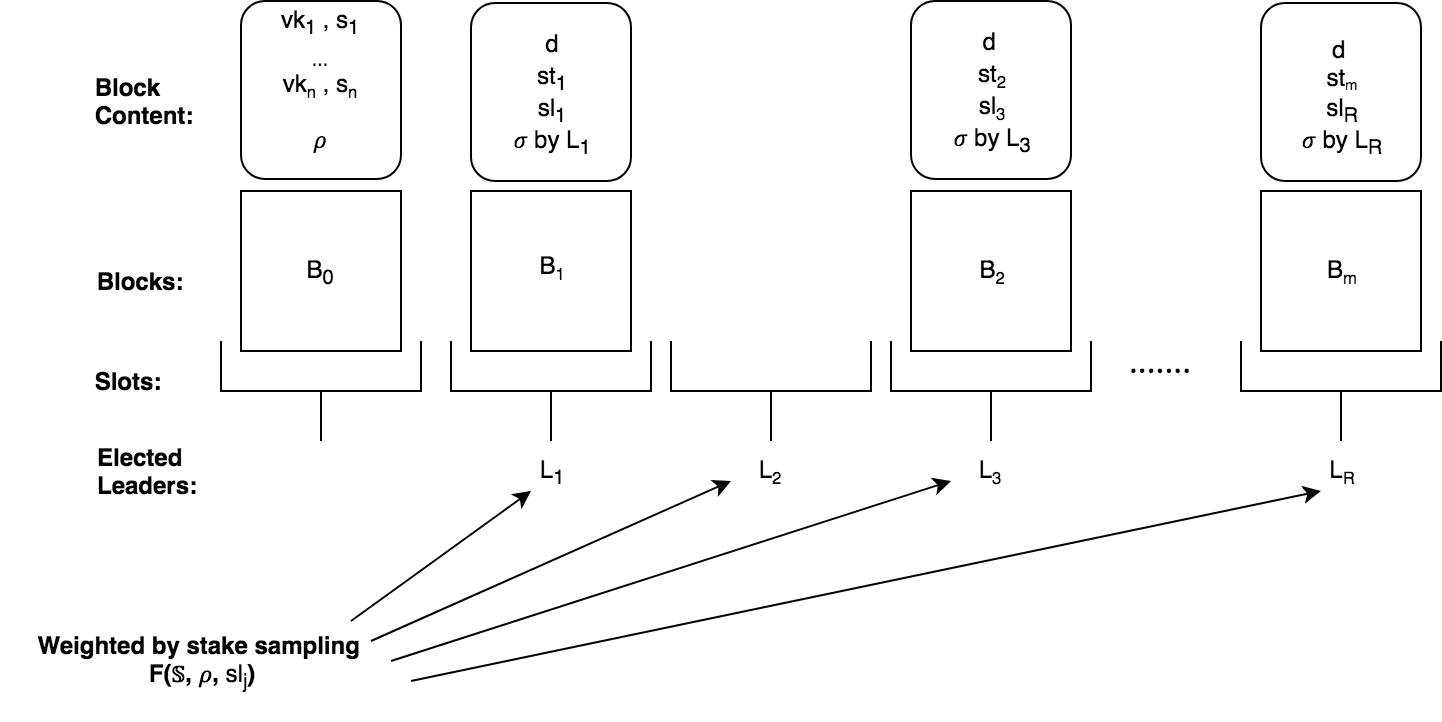
\includegraphics[width=\linewidth]{images/ouroboros-chain.png}
    \caption{Ouroboros chain structure}
    \label{fig:ouro-chain}
\end{figure}

This construction hinges on the randomness of the genesis block. Intuitively if a malicious party were able to determine this randomness, he would also be able to determine the leader election process, resulting in full control for the malicious party. 

For the first incremental analysis done in \cite{ouroboros}, a randomness beacon is utilized to show security given the random $seed$ in each epoch. This construction is shown in figure \ref{fig:ouro-epoch}.

\begin{figure}[H]
    \centering
    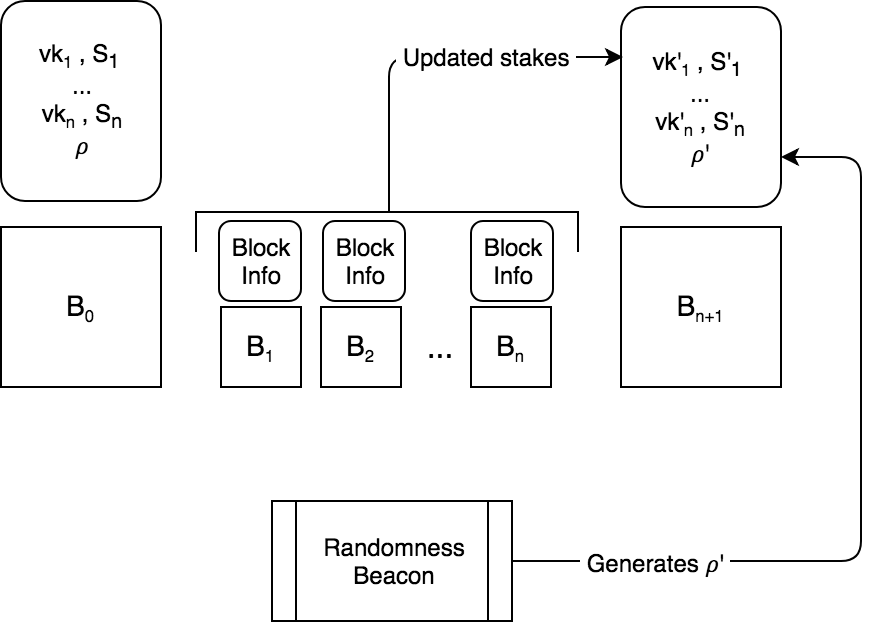
\includegraphics[width=\linewidth]{images/Ouroboros-epoch.png}
    \caption{Ouroboros with two epochs}
    \label{fig:ouro-epoch}
\end{figure}

This randomness beacon is seen as a trusted party, which cannot be dependent upon in a real setting. So a sub-protocol called Guaranteed Output Delivery (G.O.D.) Coin Tossing for generating this randomness is used. The guaranteed output is required, as if a malicious party did not like the output of the randomness calculated, he could simply abort the process and thereby the process will be rerun until the malicious party is satisfied.

It uses cryptographic primitives explained in the preliminaries, chapter \ref{cha:Preliminaries}. Notably the verifiable secret sharing and coin tossing scheme. 

The protocol is run by a subset of elected stakeholders each one corresponding to a slot during an epoch $e_j$, that lasts $R = 10k$ slots. These stakeholders are denoted $U_1, \dots, U_R$. The G.O.D coin flipping protocol consists of 3 phases; a commitment phase lasting $4k$ slots, reveal phase lasting $4k$ slots and a recovery phase lasting $2k$ slots. 


\begin{enumerate}
    \item \textbf{Commitment Phase:} At the beginning of epoch $e_j$, more precisely the first $4k$ slots, stakeholder $U_i$ for $1\leq i \leq n$ samples a string $u_i$ and randomness $r_i$ at uniformly random, and then computes commitments $Com(r_i, u_i)$. $U_i$ then computes shares $\sigma_1^i,\ldots, \sigma_n \xleftarrow{} Deal(n,u_i)$, which are then encrypted under the public-key of stakeholder $U_k$. The last part of this phase is for $U_i$ to post the encrypted shares and the commitments to the blockchain.   
    \item \textbf{Reveal Phase:} After the $4k$ slots in the commitment phase, each stakeholder $U_i$ opens its commitment with $open(r_i, u_i)$ to the blockchain provided that the blockchain contain valid shares from the majority of $U_1,\dots, U_R$ otherwise it terminates.
    \item \textbf{Recovery Phase:} In the last $2k$ slots any stakeholder $U^a$ that did not participate in the reveal phase, submits its share $\sigma^a_i$ for insertion to the blockchain. When all shares are available each stakeholder can reconstruct $u_a$, which is the new random seed, from $Rec(\sigma^a_1, \dots, \sigma^a_n)$.
\end{enumerate}



\subsection{Analysis}
\label{sec:ouro-anal}

In order to formalize the above protocol in an analyzis, some definitions about the security model are required. For the analyzis, an overview of the model will be introduced, along with some necessary definitions in order to show common prefix, chain quality, and chain growth. The analysis in \cite{ouroboros} is expanded upon in four stages showing its security under each of them. The first stage is using a static stake, the second stage uses epochs and thus having a dynamic stake but using a trusted beacon to create randomness, stage three will exchange the beacon with the G.O.D coin flipping protocol and stage four augments the protocol by introducing input-endorsers, stakeholder delegates and anonymous communication.\\

The primary focus within this thesis will be on the static stake model, while making brief notes on the dynamic stake and of the G.O.D coin flipping protocol.

\paragraph{Static stake} The static stake has from the genesis block a hardcoded initial stake distribution, with the initial set of $n$ stakeholders which are identified by their public key i.e., $\{vk_i, s_i\}_{i=1,...,n}$. It is assumed there is an honest majority with an advantage $\epsilon > 0$ s.t. there is a maximum of $\frac{1-\epsilon}{2}$ adversarial stake. It is noted that corruption is done by providing a party $U$ a corrupt token and that the corruption delay is the same as the lifetime of the system. So corruption is static in this setting, i.e., parties are corrupted from the beginning.

\subsubsection*{Model}

%% Environment
The model in which the protocol is analyzed the same as the one described in the analysis of Bitcoin \ref{subsec:anal-bitcoin}, but enhanced with an ideal functionality $F$. This functionality $F$ uses the standard model over random oracle model explained in the bitcoin analysis \ref{subsec:anal-bitcoin}. To sum up for completeness; $VIEW_{\Pi, A, \mathcal{Z}}^{P,F}$ denotes the view of a party $P$ after the execution of protocol $\Pi$ with adversary $A$ by the environment $\mathcal{Z}$, with security parameter $\kappa$ and access to the functionality $F$. $EXEC_{\Pi, A, \mathcal{Z}}^{P,F}(\lambda)$ denotes the output to the environment $\mathcal{Z}$ on the input $\lambda$.\\

%% Functionalities
For the analysis two functionalities are used; the \emph{diffuse} functionality, $F_D$, represents how messages are distributed throughout the network, and the \emph{key and transaction functionality}, $F_{KT}$, covers maintaining keys for all parties. They are defined as follows:

\paragraph{Diffuse functionality} maintains incoming strings for each party $U_i$ that participates. If a party is activated, it can fetch the contents of the incoming strings. The parties can also distribute or \emph{diffuse} a message, in which case the message is appended to the other parties incoming string. It also maintains rounds (also referred to as slots) and all parties must diffuse once in a round in order for the rounds to advance. Adversaries can additionally read all messages as well as changing the order of the messages for all other parties, but cannot stop messages from reaching a party. The current round(or slot) may at any time be requested from a party, and if the parties do not fetch the contents of their incoming strings, they are flushed after the round. 

\paragraph{Key and Transaction functionality} is initialized with $n$ users $U_1, \dots, U_n$ along with their stake $s_1,\dots, s_n$. After the initialization, the functionality can be contacted by the adversary and accepts a sequence of $(Corrupt, U_i)$ tokens, and will mark those users $U_i$ as corrupt. The adversary will then set the public keys for the corrupt users. For the honest users, the functionality will sample public/secret-key pairs and record them based on a digital signature algorithm.
\begin{itemize}
    \item A user may request to retrieve its public and secret-key.
    \item A user may request all public keys.
    \item A new user can be created by a message $(Create, U, C)$ from the environment. Upon creation, the adversary will be consulted about its corruption status, and if corrupted the adversary can set the keys. Additionally, it will store chain $C$ as its initial state. Upon creation, the public-key will be returned to the environment. Note creating new users has no impact on the protocol in the static setting.
    \item An existing user can request to be corrupted by the adversary via a message $(Corrupt, U)$. This corruption is done after a delay of $D$ slots according to the round counter from the Diffuse functionality. This delay is in the static setting the same as the lifetime of the system.
\end{itemize}

Note: These functionalities are jointly referred to as a singular functionality $F_{D+KT}$.\\

Additionally, when parties are activated during execution of the protocol the following hold:

\begin{itemize}
    \item At each slot $sl_j$, the environment $\mathcal{Z}$ is allowed to activate any subset of stakeholders it wishes. Each with a possibility of producing messages that are transmitted to other stakeholders. 
    \item After each slot $sl_j$ the adversary is activated as the last entity.
\end{itemize}


% Restriction of the environment.
This gives the adversary a lot of power, so in order to guarantee security, three restrictions will be imposed on the environments.
\begin{enumerate}
    \item In every slot at least one honest party will be activated.
    \item There is a parameter $k \in \mathbb{Z}$ that will signify maximum number of slots and honest shareholders can be offline. Given a newly spawned honest stakeholder through $(Create, U, C)$ its initialization chain should match that of the previously activated honest parties chain.
    \item Given a total stake of $\sum s_i$, the total adversarial stake of the corrupted keys is less than $50\%$ in all possible $\mathbb{S}_j(r)$. Where $\mathbb{S}_j(r)$ is a set of public keys of the form $(vk_i, s_i) \in \{0,1\}^* \times \mathbb{N}$, for $j=1,...,n_r$, where $n_r$ is the stakeholders introduced before that slot. If the adversary owns more than $50\%$ of the stake an event called $BAD^{1/2}$ becomes true.
\end{enumerate}

The second restriction is stated to be very conservative, and the protocol can handle longer offline times for a party. However, for simplicity, the above restriction is made. Secondly, the third restriction assuming honest majority is used throughout the proofs in the paper. So proofs in the paper are made that \emph{some} property $Q$ holds with high probability means $Q \text{ or } BAD^{1/2}$ with high probability.


% Introduce ISPos and argue indistinguishable from SPOS
The static stake protocol is explained in a simplified manner in the previous design section, as such the formalized version of the protocol is omitted in this section. For reading the formalized protocol $SPoS$, see \cite{ouroboros}. $SPoS$ is not used in the formal analysis, but an ideal version, called $iSPoS$, where abstraction of the cryptographic primitives into \emph{functionalities} is used. Proposition 4.8 in \cite{ouroboros} shows that the view of the execution of the static stake protocol, $SPoS$, and the ideal static stake protocol, $iSPoS$, are computationally indistinguishable. As such all further analysis is done on $iSPoS$. $iSPoS$ is run by stakeholders $U_1,\dots,U_n$ who are interacting with $\mathcal{F}_{LS}^{\mathcal{D},F}[\mathcal{F}_\text{DSIG}]$ over $S=\{sl_1\,\dots,sl_R\}$, and proceeds as defined in \cite{ouroboros}:
\begin{enumerate}
    \item \textbf{Initialization} Stakeholder $U_i \in \{U_1, \dots, U_n\}$ receives from the key registration interface its public and secret key. Then it receives the current slot from the diffuse interface and in case it is $sl_1$ it sends $(genblock_req, U_i)$ to $\mathcal{F}_{LS}^{\mathcal{D},F}[\mathcal{F}_\text{DSIG}]$, receiving $(genblock,\mathbb{S}_0, \rho, F)$ as answer. $U_i$ sets the local blockchain $C= B_0 = (\mathbb{S}_0, \rho)$ and the initial internal state $st=H(B_0)$. Otherwise, it receives from the key registration interface the initial chain $C$, sets the local blockchain to $C$ and the initial internal state $st=H(\text{head}(C))$.
    
    \item \textbf{Chain Extension} For every slot $sl_j \in S$, every stakeholder $U_i$ performs the following steps:
    \begin{enumerate}
        \item Collect all valid chains received via broadcast into a set $\mathbb{C}$, verifying that for every chain $C'\in \mathbb{C}$ and every block $B'=(st',d',sl',\sigma') \in C$ it holds that $\mathcal{F}_\text{DSIG}$ answers with $(\text{Verified}, sid, (st',d',sl'),1)$ upon being queried with \\ $(\text{Verify}, sid, (st',d',sl'), \sigma', vk')$, where $vk'$ is the verification key of the stakeholder $U'=F(\mathbb{S}_0,\rho,sl')$. $U_i$ computes $C'=\text{maxvalid}(C, \mathbb{C})$, sets $C'$ as the new local chain and sets state $st=H(\text{head}(C'))$.
        \item If $U_i$ is the slot leader determined by $F(\mathbb{S}_0,\rho,sl_j)$, it generates a new block $B=(st,d,sl_j,\sigma)$ where $st$ is the current state, $d\in\{0,1\}^{*}$ is the transaction data and $\sigma$ is obtained from $\mathcal{F}_\text{DSIG}$'s answer $(\text{Signature}, sid, (st,d,sl_j), \sigma)$ upon being queried with $(\text{Sign}, sid_i, (st,d,sl_j))$. $U_i$ computes $C' = C|B$, broadcasts $C'$, sets $C'$ as the new local chain and sers state $st=H(\text{head}(C'))$.
    \end{enumerate}
    
    \item \textbf{Transaction generation} Given a transaction template $tx$, $U_i$ returns $\sigma$ obtained from $\mathcal{F}_\text{DSIG}$'s answer $(\text{Signature}, sid_i, tx, \sigma)$ upon being queried $(\text{Sign}, sid_i, tx)$, provided that $tx$ is consistent with the state of the ledger in the view of $U_i$.
\end{enumerate}


\subsubsection*{Forkable Strings}

% Forkable Strings
For analyzing the protocol with regard to \emph{common prefix, chain quality} and \emph{chain growth} the notion of \emph{forkable strings} has to be introduced. To determine what a forkable string is, a \emph{characteristic string} and a \emph{fork} has to be defined. Intuitively, the characteristic string is on form $\{0,1\}^n$ and used to indicate whether or not the slots have been assigned to adversarial stakeholders. A formal definition of a characteristic string is defined in \cite{ouroboros} and is as follows.

%% Def Characteristic String
\begin{mydef}[Characteristic String]
\label{def:char-string}
Fix an execution with genesis block $B_0$, adversary $A$, and environment $\mathcal{Z}$. Let $S = \{ sl_{i+1}, \ldots sl_{i+n} \}$ denote a sequence of slots of length $|S| = n$. The characteristic string $w \in \{0,1\}^n$ of $S$ is defined so that $w_k = 1$ if and only if the adversary controls the slot leader of slot $sl_{i+k}$. For such a characteristic string $w\in \{0,1\}^{*}$ we say that the index $i$ is adversarial if $w_i = 1$ and honest otherwise.
\end{mydef}

A concern regarding characteristic strings is outlined in the following example. If two honest parties both go offline with view $C_0$, when they come back online and requesting an update to their chain, then an adversary can force them to adopt two different chains $C_1$ and $C_2$, whose common prefix is $C_0$. This kind of \emph{forking} is defined in \cite{ouroboros} as follows.

%% Def Fork
\begin{mydef}[Fork]
Let $w\in \{0,1\}^n$ and let $H=\{ i | w_i=0 \}$ denote the set of honest indices. A fork for the string $w$ is a directed, rooted tree $F = (V,E)$ with a labeling $\ell \xrightarrow{} \{0,1,\ldots,n\}$ so that
\begin{itemize}
    \item each edge of $F$ is directed away from the root;
    \item the root $r\in V$ is given the label $\ell(r)=0$;
    \item the labels along any directed path in the tree are strictly increasing;
    \item each honest index $i\in H$ is the label of exactly one vertex of $F$;
    \item the function $\textbf{d} : H\xrightarrow{} \{1,\ldots,n\}$, defined so that $\textbf{d}(i)$ is the depth in $F$ of the unique vertex $v$ for which $\ell(v)=i$, is strictly increasing. (Specifically, if $i,j\in H$ and $i<j$, then $\textbf{d}(i) < \textbf{d}(j)$.)
\end{itemize}
\end{mydef}

Furthermore, a fork can be considered flat if it contains two tines, which do not share an edge and are of a length equal to the height of the fork. A tine is defined as a path originating from the root, and the length of a tine denoted $length(t)$, is the number of edges on the tine.
An example on a forkable string can be seen in figure \ref{fig:forkable_string}. The characteristic string $w = 010100110$ is forkable, which is shown by the directed tree $F$ and denoted by $F \vdash w$. In $F$ each vertex with double borders is honest, where the vertex with single border is adversarial. One notable remark is that the depth of honest vertices associated with the indices of $w$ is strictly increasing. 

\begin{figure}
    \centering
    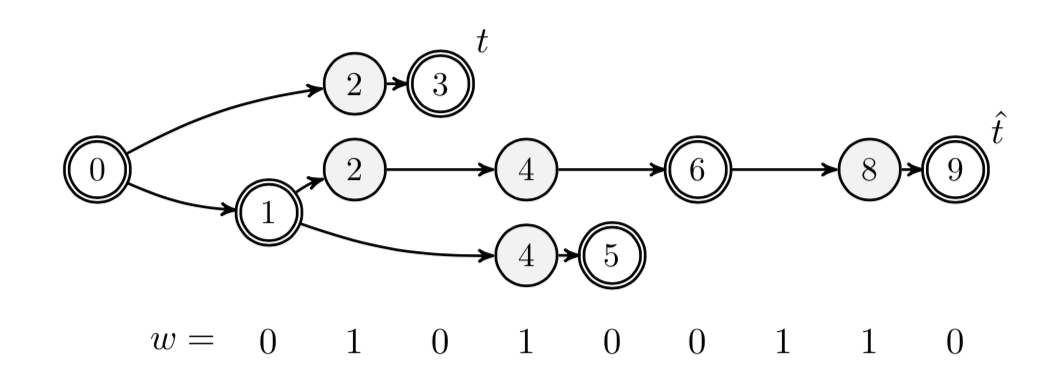
\includegraphics[width=\linewidth]{images/ouro-forkable-string.png}
    \caption{Forkable string}
    \label{fig:forkable_string}
\end{figure}

The directed tree $F$ in figure \ref{fig:forkable_string} contains two distinguished tines, namely $t$ and $\hat{t}$. Furthermore, two tines can share an edge and it is denoted by $t_1 \sim t_2$. In figure \ref{fig:forkable_string} the length of $F$ is six, since the length of a fork is defined to be the length of the longest tine. $F$ is considered to be closed, due to all the leafs of $F$ is honest. 

In \cite{ouroboros} they show that a string $w$ is forkable iff there is a closed fork $F$ such that $margin(F) \geq 0$. The margin is defined to be the second last reach taken where $t_1 \not\sim t_2$, where the reach is defined as:
\begin{equation}
\label{eq:ouro-reach}
    reach(t) = reserve(t) - gap(t)
\end{equation}
In equation \ref{eq:ouro-reach}, the \emph{reserve} is defined to be the amount of adversarial indices of $w$ after the last index in the tine $t$. The \emph{gap} is defined to be the difference in length of the tines $t$ and another tine $\hat{t}$. More formally, the margin of a fork $F$ is defined in \cite{ouroboros} as:
\begin{equation}
    margin(F) = max_{t_1 \not\sim t_2}(min\{reach(t_1),reach(2)\})
\end{equation}

% Covert adversaries
In section \ref{sec:ouro-cpcqcg}, the common prefix is shown with regard to traditional adversaries and covert adversaries. Covert adversaries differ from the traditional adversaries in the following way. A traditional adversary has the possibility of broadcasting multiple blocks within a single slot, and thereby it can extend multiple chains. If a traditional adversary chooses to broadcast multiple blocks within a given slot, then the adversary leaves a trail of acting maliciously, due to multiple signed blocks. For a more stealthy adversary, the covert adversary is only broadcasting one block per slot. Though the covert adversary is only broadcasting one block per slot, it can still behave maliciously and deviate from the protocol, but it does not leave any evidence, which makes it possible to deny the malicious behavior due to the possibility of a network delay.

%Covert forks
The covert adversaries can do covert forks on strings that are covertly forkable. A characteristic string is said to be covertly forkable if and only if a majority of its indices are adversarial, and if there is a flat fork for the characteristic string. A covert fork for a covertly forkable characteristic string is defined in \cite{ouroboros} as the following.

\begin{mydef}
Let $F \vdash w$ be a fork for a string $w\in \{0,1\}^{*}$. We say that $F$ is covert if the labeling $\ell : V \xrightarrow{} \{0,1,\ldots\}$ is injective. In particular, no adversarial index is labeled by more than one node.
\end{mydef}


\subsubsection*{Common Prefix, Chain Quality and Chain Growth}
\label{sec:ouro-cpcqcg}

%% Common Prefix: Theorem 4.27 (adversarial violation in iSPoS)

\begin{theorem}[Common prefix]
\label{th:common-prefix}
    Let $k,R \in \mathbb{N}$ and $\epsilon \in (0,1)$. The probability that $\pi_{iSPoS}$ protocol, when executed with a $(1-\epsilon)/2$ fraction of adversarial stake, violates the common prefix property with parameter k throughout an epoch of $R$ slots is no more than $e^{-\Omega(\sqrt{k})+\text{ln} R}$; the constant hidden by the $\Omega()$ notation depends only on $\epsilon$.
\end{theorem} 

% Intuition of proof + mention theorem 4.26 and definition 4.25

The proof from \cite{ouroboros} assumes that $\pi_{iSPoS}$ violates the common-prefix property when the fork $F$, has $div(F) \geq k$ in an execution. $div(F)$ is defined as the divergence of $F$ as the maximum over all pairs of viable tines i.e. 

\begin{equation}
\label{eq:divF}
    div(F) = \max_{t_1, t_2} \: div(t_1, t_2)
\end{equation}

In equation \ref{eq:divF} the divergence of two viable tines in F is defined as

\begin{equation}
\label{eq:divergence}
    div(t_1, t_2) = \underset{i}{\min} \: (length(t_i) - length(t_1 \cap t_2))
\end{equation}

In equation \ref{eq:divergence} the notation $t_1 \cap t_2$ refers to the common prefix of $t_1$ and $t_2$. The notation is additionally overloaded given a characteristic string as defined in definition \ref{def:char-string} s.t. $div(w) = \underset{F \vdash w}{\max} \: div(F)$. \\

To prove the common prefix theorem, it needs to shown that \\ $Pr[div(w) \geq k] \leq e^{-\Omega(\sqrt{k}+ \text{Ln} R)}$, in which the event $div(w) \geq k$ is defined as $BAD$. 
Theorem 4.26 in \cite{ouroboros} states; \emph{let $w \in \{0,1\}^*$. Then there is a forkable substring $\hat{w}$ of $w$ with $|\hat{w}| \geq div(w)$}.

Given this theorem, there exists a forkable substring $\hat{w}$ of $w$ with length at least $k$.

\begin{align*}
\label{eq:common-pref-violation}
    &Pr[\text{Common prefix violation}]\\
    &\leq Pr[\exists \alpha, \beta \in \{1,\ldots, R\} \text{ s.t. }  \alpha + k -1 \leq \beta \text{ and } w_\alpha,\ldots, w_\beta \text{ is forkable}]\\
        &\leq \sum_{1 \leq \alpha \leq R} \bigg( \sum_{\alpha+k-1 \leq \beta \leq R} Pr[w_{\alpha}, \ldots, w_{\beta} \text{ is forkable}] \bigg) \numberthis
\end{align*}

Where $\alpha$ is defined as $\alpha \overset{\Delta}{=} \ell(y) = \ell(t_1 \cap t_2)$, and denotes the label of the last index of the common prefix of $t_1$ and $t_2$. While $\beta$ is defined as the smallest honest index of $w$ for which $\beta \leq \ell(t_2)$ if $\not\exists \beta$ then $\beta = n+1$, where it is assumed for simplicity without loss of generality that $\ell(t_1) < \ell(t_2)$.\\


Theorem 4.13 in \cite{ouroboros} states \emph{if $\epsilon \in (0,1)$ and $w \in \{0,1\}^n$ then by independently assigning each $w_i = 1$ with $(1-\epsilon)/2$. Then $Pr[w$ is forkable$]=2^{-\Omega(\sqrt{n})}$, the probability that a string of length $t$ drawn from this distribution is forkable no more than $e^{-c\sqrt{t}}$, for a positive constant $c$}.

Thus the cumulative probability of possible strings for any $\alpha \geq 1$ can be calculated with the following: 
\begin{equation}
\label{eq:com-pre-bound}
    \sum_{t=\alpha + k - 1}^{R} e^{-c \sqrt{t}} \leq e^{-\Omega(\sqrt{k})}
\end{equation}

At which the probability of a violation of the common prefix can be calculated: 
\begin{equation*}
    Pr[\text{common prefix violation}] \leq R \cdot e^{-\Omega(\sqrt{k})} \leq e^{ln R - \Omega(\sqrt{k})}
\end{equation*}
as desired.

%% Common Prefix: Theorem 4.29 (covert adversarial violation in iSPoS)
\begin{theorem}[Common prefix - covert]
\label{th:comPrefix-covert}
    Let $k,R \in \mathbb{N}$ and $\epsilon \in (0,1)$. The probability that $\pi_{iSPoS}$ protocol, when executed with a $(1-\epsilon)/2$ fraction of adversarial stake and covert adversary, violates the common prefix property with parameter k throughout an epoch of $R$ slots is no more than $e^{-\Omega(k)+\text{ln} R}$; the constant hidden by the $\Omega()$ notation depends only on $\epsilon$.
\end{theorem}

% Intuition of proof
The proof follows almost identically as the one for theorem \ref{th:common-prefix}. But utilizing theorem 4.28 from \cite{ouroboros} that covers covertly forkable substrings instead of the aforementioned theorem 4.26 from \cite{ouroboros} and theorem 4.23 from \cite{ouroboros} instead of the aforementioned theorem 4.13 from \cite{ouroboros}.

%% Chain Growth: Theorem 4.31
\begin{theorem}[Chain growth]
    The $\pi_{iSPoS}$ protocol satisfies the chain growth property with parameters $\tau = 1- \alpha, s \in \mathbb{N}$ throughout an epoch of $R$ slots with probability at least $1 - e^{-\Omega(\epsilon^2s) +\text{ln} R}$ against an adversary holding an $\alpha - \epsilon$ portion of the total stake.
\end{theorem}

% Intuition of proof 
First, the event that the Hamming weight ratio of $w$ that corresponds to the slots $[a,a+s-1] \leq \alpha$ is denoted $Ham_a(\alpha)$. To clarify, the hamming weight is the number of characters in a string not being 0 i.e. owned by a malicious party.

For each slot the adversary has a probability of $\alpha - \epsilon$ to be assigned to the given slot, due to holding $\alpha-\epsilon$ of the total stake. From this the probability that the Hamming weight ratio is more than $\alpha s$ drop exponentially in $s$. From the additive Chernoff-Hoeffding bound, $Pr[\sum_i^n x_i \geq np + n\epsilon] \leq exp(-2n\epsilon^2)$, equation \ref{eq:ham-chernoff} follows 

\begin{align*}
\label{eq:ham-chernoff}
    Pr\left[\sum_i^s x_i \geq s\alpha + s\epsilon\right] = \; &Pr[\neg Ham_a(\alpha)] \leq e^{-2 \epsilon^2 s} \\
    \implies &Pr[Ham_a(\alpha)] \geq 1 -e^{-2 \epsilon^2 s} \numberthis
\end{align*}

From equation \ref{eq:ham-chernoff}, whenever the event $Ham_a(\alpha)$ happens, then in a period of $s$ rounds there will be at least $(1-\alpha)s$ slots which are honest. This gives that the blockchain will advance by at least $(1-\alpha)s$ blocks if for each slot, an honest party produces a block. Due to the union bound, the parameter $\tau$, which denotes the speed coefficient, can be set to $1-\alpha$, which is satisfied with probability at least $1-e^{-2\epsilon^2 s + \ln R}$.



%% Chain Quality: Theorem 4.32
\begin{theorem}[Chain quality]
    Let $\alpha - \epsilon$ be the adversarial stake ratio. The $\pi_{iSPoS}$ protocol satisfies the chain quality property with parameters $\mu(\alpha - \epsilon) = \alpha/(1 - \alpha)$ and $\ell \in \mathbb{N}$ throughout an epoch of $R$ slots with probability at least $1-e^{-\Omega(\epsilon^2\alpha \ell)+\text{ln} R}$
\end{theorem}

% Intuition of proof
From the chain growth theorem it follows that there is a high probability of a segment of $\ell$ rounds, which will contain at least $(1 - \alpha) \ell$ slots from a honest majority. Given a honest party always advances the chain, the chain will advance with $(1 - \alpha) \ell$ blocks during the segment of $\ell$ rounds and likewise the dishonest parties will not have more than $\alpha \ell$ blocks. Thus it follows from a chain held by a honest party it will contain a fraction $\alpha/(1 - \alpha)$ of adversarial blocks with probability 
\begin{equation*}
    1 - e^{- \Omega(\epsilon^2 \min(\alpha, 1- \alpha)\ell)+ ln \: R}
\end{equation*}


\subsubsection*{Extension to epochs}
The above protocol only covers a static stake running a single epoch following the algorithm. This means coins changing through the execution of this epoch does not affect the slot leader selection. To extend this to a dynamic stake, the protocol is extended into multiple epochs. For each epoch, the genesis block which contained the randomness and stake of the given peers is updated, thus also affecting the slot leader election. For this the functionality $\mathcal{F}^{D,F}_{DLS}$ is extended with a \emph{genesis block generation} functionality, along with \emph{epoch randomness update} functionality, which samples the randomness for the epoch. This represents the functionality of the randomness beacon described previously. Note for the extension from the passive protocol the stakeholders will need to request the randomness from the epoch randomness update functionality at the beginning of each epoch.

\subsubsection*{Replacement of randomness beacon}
In the previous section, the protocol was extended into multiple epochs along with an introduction of the randomness beacon. In \cite{ouroboros}, an implementation of the randomness beacon, denoted $\pi_{DLS}$, will make use of a few cryptographic primitives known from the field of \emph{multi-party computation}, namely a \emph{coin tossing protocol} and a \emph{verifiable secret sharing scheme}, see chapter \ref{cha:Preliminaries} for definitions. The general idea of $\pi_{DLS}$ is to generate unbiased randomness by using the coin tossing protocol, but an adversary could make the protocol fail by aborting it. By having this concern, $\pi_{DLS}$ also makes use of a verifiable secret sharing scheme, and by this combination of a coin tossing protocol and a verifiable secret sharing scheme, $\pi_{DLS}$ becomes a coin tossing protocol with guaranteed output delivery.

\begin{figure}[H]
    \centering
    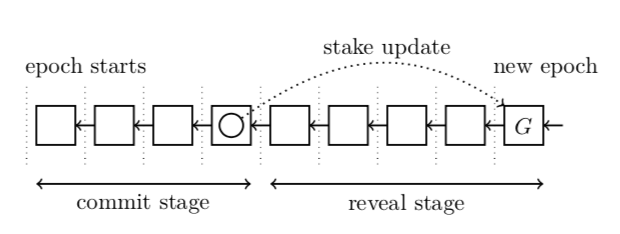
\includegraphics[scale=0.75]{images/ouro-commit-reveal.png}
    \caption{The guaranteed output delivery protocol's two stages for generating randomness}
    \label{fig:ouro-commit-reveal}
\end{figure}

In figure \ref{fig:ouro-commit-reveal}, the two stages of $\pi_{DLS}$ is seen. In the commit stage, the commitment of the coin tossing protocol and the shares of the verifiable secret sharing scheme is sampled. Furthermore, the commit is posted to the blockchain along with the encryptions of all the shares, which are encrypted under the public-key of each respective shareholder. The reveal stage starts when a majority of the stakeholders has posted their commitments to the blockchain, as well as shares from a majority of the stakeholders has been received. In the reveal stage, stakeholders post to the blockchain open-values to their particular commit. Lastly, a \emph{recovery phase} is entered, where each stakeholder with respect to the verifiable secret sharing scheme computes the common random seed to the leader election. 


% Praos  
\section{Ouroboros Praos}

\subsection{Design}

The Ouroboros Praos protocol \cite{ouroboros-praos}, also simply refered to as \emph{Praos}, relies on two cryptographic functions; \emph{Verifiable Random Functions}, abbreviated $VRF$ and \emph{Key Evolving Signatures}, abbreviated $KES$, which are both described in section \ref{cha:Preliminaries}. As well as digital signatures described in subsection \ref{subsec:Digital-signature}, here abbreviated to $DSIG$. 

The protocol is executed among $U_1,\dots, U_n$ stakeholders over a sequence of slots $S = \{sl_1, \dots, sl_R\}$. In Praos each slot is not limited to a single possible block, but can have none or multiple leaders. Praos consists of three parts; \emph{Initialization}, \emph{Chain Extension} and \emph{Signing Transactions}.

\paragraph{Initialization} A stakeholder $U_i$ generates keys of $VRF, KES, DSIG$. The public keys $v^{VRF}_i$ for the verifiable random function, $v^{KES}_i$ for the key evolving signature and the $v^{DSIG}_i$ for the digital signature, will be contained in the genesis block along with the stakeholders stake $s_i$. Creating the genesis block $\mathbb{S}_0 = (U_i, v_i^{vrf}, v_i^{kes}, v_i^{dsig}, s_i)$ for $i = \{1, \dots, n\}$ along with initial randomness in the form of a nonce $\eta$. All $U_i$ initialized in the first round set $(\mathbb{S},\eta)$ to $B_0$ and state $st = H(B_0)$. With H being a collision resistant hash function as defined in the preliminaries, section \ref{def:hash}. If a stakeholder $U_i$ was initialized later, it sets its state $st = H(Head(C))$, with C being the longest chain.

\paragraph{Chain Extension} After initialization, every stakeholder $U_i$ performs the following steps for every slot $sl_j \in S$
\begin{enumerate}
    \item The stakeholder $U_i$ receives transaction data $d \in \{0,1\}^*$ from the users in the network that want to append to the blockchain.
    
    \item The stakeholder $U_i$ collects all valid chains received from the network into a set $\mathbb{C}$ and verifies every chain $C' \in \mathbb{C}$. $U_i$ verifies that every block $B'=(st',d',sl',B_{\pi}',\sigma_j') \in C'$ is created by the correct slot leader in $sl'$, as well as verifying the key evolving signature. After verifying the chains the stakeholder $U_i$ computes $C' = maxvalid(C, \mathbb{C})$ and sets the new local chain to $C'$ and the state $st = H(head(C'))$. Note: $maxvalid(C, \mathbb{C})$ gives the longest chain from $\mathbb{C} \cup \{C\}$, and if there are two longest chains, one of them is chosen randomly.
    
    \item The stakeholder $U_i$ lastly checks if he owns the slot $sl_j$ by checking if the output $y$ of the function $VRF$ is below \emph{some} threshold $T_i$. $T_i$ is based on the individual stake of the stakeholder, and thereby defining the probability of the stakeholder to be elected as the leader for a given slot. If the stakeholder's $y$ is below the threshold, he can create a new block $B = (st, d, sl_j, B_{\pi}, \sigma)$, with $d$ being data, $sl_j$ being the slot, $B_{\pi} = (U_i, y, \pi)$ being the block proof from $VRF$, the key evolving signature $\sigma$ and lastly setting the state $st = H(head(C|B))$. $U_i$ sets his local chain to be the newly created chain and broadcasts it to the network.
\end{enumerate}

\paragraph{Signing Transactions} To make a transaction a user signs the transaction with his digital signature, and broadcasts ($tx, \sigma$).

In figure \ref{fig:praos-epochs} an illustration of the protocol is provided, which shows the overall structure of the protocol. The protocol much resembles the original Ouroboros structure in which, each peer generates blocks in designated slots. The big difference here is the randomness generating function for the nonce of the next epoch. Here it uses the previous nonce, the epoch number and the random values $y_1, \dots, y_{8k}$ from $VRF$, and a hash function for generating the next nonce.

\begin{figure}[H]
    \centering
    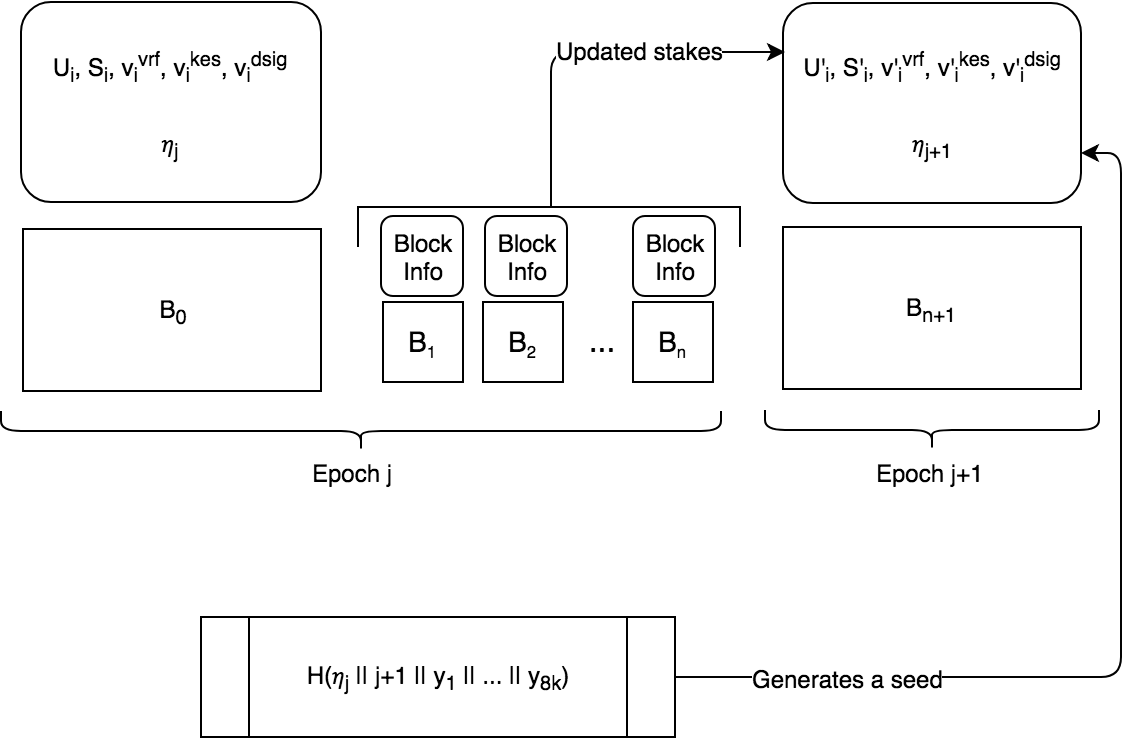
\includegraphics[width=\linewidth]{images/Praos-epoch.png}
    \caption{Two epochs within the Praos protocol.}
    \label{fig:praos-epochs}
\end{figure}

\subsection{Analysis}

The analysis of Ouroboros Praos is heavily influenced by the Ouroboros protocol and the analysis of the backbone protocol in section \ref{subsec:anal-bitcoin}.

%% Security Model
As such many definitions for the \emph{common prefix}, \emph{chain growth} and \emph{chain quality} properties, as well as the model remains mostly the same with some slight alterations. Instead of repeating the whole model described in section \ref{sec:ouro-anal}, only the modifications will be described here.\\

In Praos two additional properties that the protocol wants to capture is adversarial-controlled message delays by $\Delta \in \mathbb{N}$ and immediate adaptive corruption. The model also uses the same definition of how \emph{time} is sorted into discrete units called \emph{slots}. 

%% Functionalities

The protocol makes heavy use of functionalities to abstract the cryptographic primitives used throughout the protocol. The first functionality called Delayed Diffuse functionality, $\mathcal{F}_{DDiffuse_{\Delta}}$, is for abstracting the underlying network.

\paragraph{Delayed Diffuse functionality} To capture the adversarially-controlled message delays, another variation of the Diffuse functionality is used, namely the \emph{Delayed diffuse functionality} denoted $\mathcal{F}_{DDiffuse_{\Delta}}$. It takes the parameter $\Delta \in \mathbb{N}$, and executes a round per slot. The functionality interacts with the environment $\mathcal{Z}$ and the stakeholders $U_1, ..., U_n$ and adversary $A$.
\begin{itemize}
    \item For each party $U_i$ the functionality maintains a string. At any moment the party $U_i$ is allowed to fetch its strings and in each round $U_i$ is allowed to diffuse a message.
    \item Upon activation, the adversary $A$ is allowed to do three things.
    \begin{itemize}
        \item Read all inboxes messages, diffuse requests and order messages as he chooses.
        \item $A$ can choose to put a message $m$ into a special $delayed_i$ string, instead of putting it into the inbox of $U_i$.
        \item The adversary $A$ can insert a message from $delayed_i$ into the inbox of a stakeholder $U_i$.
    \end{itemize}
    \item At the end of each round the functionality makes sure all diffused messages that were not put into $delayed_i$ or messages removed from $delayed_i$ is inserted into the inbox of the stakeholder $U_i$. If a message $m$ has been in the $delayed_i$ for at least $\Delta$ it is moved to the inbox of $U_i$.
    \item Receiving (Create, U, C) from the environment, the functionality spawns a new stakeholder with local chain $C$.
\end{itemize}

To further abstract the cryptographic building blocks into functionalities three additional functionalities are described for \emph{Digital Signatures} denoted $\mathcal{F}_{DSIG}$, \emph{Key Evolving Signature} denoted $\mathcal{F}_{KES}$ and \emph{Verifiable Random Function} denoted $\mathcal{F}_{VRF}$.

% From appendix A.2
% is U_i correct in keyGen?
\paragraph{Digital Signature functionality} $\mathcal{F}_{DSIG}$ interacts with a signer $U_S$ and stakeholders $U_1, \dots, U_n$. 
\begin{itemize}
    \item \textbf{Key Generation} Upon receiving ($KeyGen, sid, U_s$) from a stakeholder $U_s$, forward the triple to the adversary, in which the adversary responds with $(VerificationKey, sid, U_s, v)$. Output ($VerificationKey, sid, v$) to $U_i$ and record the triple ($sid, U_s, v$).
    \item \textbf{Signature Generation} When the functionality receives \\ ($Sign, sid, U_s, m$) from a stakeholder $U_S$, verify the triple for $U_S$ has been recorded. Then send ($Sign, sid, U_s, m$) to the adversary which will return ($Signature, sid , U_s, m, \sigma$), verify that there is no entry ($m, \sigma, v, 0$) recorded, if not record the entry ($m, \sigma, v, 1$)
    \item \textbf{Signature Verification} Upon receiving a message \\ ($Verify, sid, m, \sigma, v'$) from a stakeholder $U_i$ forward it to the adversary. When receving ($Verified, sid, m, \varphi$) do one of the following:
    \begin{enumerate}
    % Completeness: If the verification key v′ is the registered one and σ is a legitimately generated signature for m, then the verification succeeds
        \item if $v' = v$ and ($m, \sigma, v, 1$) is recorded set $f = 1$ 
    % Unforgeability: If v′ is the registered one, the signer is not corrupted, and never signed m, then the verification fails.
        \item else if $v' = v$, the signer is not corrupt, and no entry ($m, \sigma', v, 1$) is recorded set $f = 0$ and record the entry \\ ($m, \sigma, v, 0$)
    % Consistency: All verification requests with identical parameters will result in the same answer.
        \item else if there is a record ($m, \sigma, v', f'$), then let $f = f'$
        \item else, $f = \varphi$ and record $(m, \sigma, v', \varphi)$.
    \end{enumerate}
    return ($Verified, sid, m, f$) to $U_i$.
\end{itemize}

\paragraph{Key Evolving Signature functionality} $\mathcal{F}_{KES}$ is parameterized by a number of signature updates $T$. It Interacts with a signer $U_S$ and the stakeholders $U_1, \dots, U_n$ in the following 3 ways:
\begin{itemize}
    \item \textbf{Key generation} Upon receiving $(KeyGen, sid, U_S)$ from a stakeholder $U_S$, forward it to the adversary. The Adversary responds with $(VerificationKey, sid, U_S, v)$ to the functionality in which the functionality returns ($VerificationKey, sid, v$) to the stakeholder, records ($USign, U_S, v$) and sets the the counter $k_{ctr} = 1$
    \item \textbf{Sign and Update} Upon receiving a message ($USign, sid, U_S, m, j$) from the stakeholder $U_S$, verify the stakeholder that ($sid, U_S, v$) is recorded and that the counter $k_{ctr} \leq j \leq T$, if not ignore the request. Otherwise, set the counter $k_{ctr} = j + 1$ and send ($Sign, sid, U_s, m, j$) to the adversary. Upon receiving \\ ($Signature, sid, U_s, m, j, \sigma$) from the adversary verify that no other record of ($m, j, \sigma, v, 0$). If it has already been recorded, return an error to the stakeholder $U_S$ and halt. Otherwise, send ($Signature, sid, m, j, \sigma$) to $U_s$ and record the entry $(m, j, \sigma, v ,1)$.
    \item \textbf{Signature Verification}. When receiving a message \\ ($Verify, sid, m, j, \sigma, v'$) from a stakeholder $U_i$ to verify the message one of the following steps are done:
    \begin{enumerate}
        \item if $v' = v$ and the entry ($m, j, \sigma, v, 1$) is recorded then set $f = 1$, this guarantees completeness.
        \item else if $v' = v$, the signer is not corrupted, and no entry ($m, j , \sigma', v, 1$) is recorded, then set $f = 0$.
        \item else if there is an entry ($m, j, \sigma, v', f'$) is recorded, then let $f = f'$.
        \item else, if $j < k_{ctr}$, let $f = 0$ and record the entry ($m, j, \sigma, v, 0$). Else, if $j = k_{ctr}$, forward ($Verify, sid, m, j, \sigma, v'$) to the adversary. When receiving ($Verified, sid, m, j, \varphi$) from the adversary let $f = \varphi$ and record the entry ($m, j, \sigma, v', \varphi$).
    \end{enumerate}
    return ($erified, sid, m, j, f$) to the stakeholder $U_i$ 
\end{itemize}

\paragraph{Verifiable Random Function functionality} $\mathcal{F}_{VRF}$ interacts with the stakeholders $U_1, \dots, U_n$ as follows:
\begin{itemize}
    \item \textbf{Honest Key Generation} On receiving the message ($KeyGen, sid$) from a honest stakeholder $U_i$ forward ($KeyGen, sid$, $U_i$) to the adversary, in which the adversary will respond with \\ ($VerificationKey, sid, U_i, v$). If $U_iS$ is honest, verify that $v$ is unique, and record ($U_i, v$), and return ($VerificationKey, sid, v$) to $U_i$ and initialize the the table $T(v, \cdot)$ to be empty.
    
    \item \textbf{Malicious Key Generation} Receiving ($KeyGen, sid, v$) from $U_S$, verify that $v$ has not been recorded. Initialize the table $T(v, \cdot)$ to be empty and record ($U_S,v$).
    
    \item \textbf{Honest VRF Evaluation} Receiving ($Eval, sid, m$) from a stakeholder $U_i$, verify that a pair ($U_i, v$) has been recorded. If $T(v,m)$ is undefined, set $y \in_R {0,1}^{\ell_{VRF}}$ and set $T(v,m) = (y, \emptyset)$ and output ($Evaluated, sid, y$) to $U_i$, where $y$ is s.t. $T(v,m) = (y,S)$ for some $S$.
    
    \item \textbf{Honest VRF Evaluation and Proof} Receiving ($EvalProve, sid, m$) from a stakeholder $U_i$, verify a pair ($U_i, v$) is recorded, then send the triple including sender to the adversary, which responds with ($Eval, sid, m, \pi$). If $T(v,m)$ is undefined verify that $\pi$ is unique and set $T(v, m) = (y,\{ \pi \})$ where $y \in_R \{0,1\}^{\ell_{vrf}}$. Otherwise append by setting $T(v,m) = (y, S \cup \{ \pi \})$. Finally output ($Evaluated, sid, y, \pi$) to $U_i$.
    
    \item \textbf{Malicious VRF Evaluation} Receiving ($Eval, sid, v, m$) from $S$ for some $v$. If ($S,v$) is recorded and $T(v, m)$ is undefined, then set $T(v,m) = (y, \emptyset)$ where $y \in_R \{0,1\}^{\ell_{VRF}}$. If, $T(v,m) = (y,S)$ for some $S \not= \emptyset$ then output ($Evaluated, sid, y$) to $S$, else ignore the request.
    
    \item \textbf{Verification} When receiving a message ($Verify, sid, m, y, \pi, v'$) from a stakeholder $U_i$, forward the message to the adversary, which will respond with ($Verified, sid, m, y, \pi, v'$). Upon receiving the message do one of the three things:
    \begin{enumerate}
        \item if $v' = v$ for some ($U_i, v$) and entry $T(U_i, m)$ equals ($y, S$) with $\pi \in S$ then set $f = 1$. 
        \item if $v' = v$ for some ($U_i, v$) but there is no entry in $T(U_i, m)$ of the form ($y, \{\dots, \pi, \dots\}$) then set $f = 0$.
        \item else initialize the table $T(v', \cdot)$ to empty and set $f = 0$.
    \end{enumerate}
    Finally the functionality outputs $(Verified, sid, m, y, \pi, f)$ to $U_i$.
\end{itemize}

The protocol also employs a Init functionality representing the generation of the genesis block, as well as a random oracle to represent the hashing functionality.

\paragraph{Init functionality} $\mathcal{F}_{INIT}$ is the functionality for initializing the genesis block. $\mathcal{F}_ {INIT}$, incorporates the diffuse functionality, $\mathcal{F}_{DDiffuse_{\Delta}}$ as mentioned previously, it is parameterized with an initial set of stakeholders $U_1, \dots, U_n$, along with their stakes $s_1, \dots, s_n$. 
\begin{itemize}
    \item In the first round, given a request ($ver_{keys}, sid, U_i, v^{vrf}_i, v^{kes}_i, v^{dsig}_i$) from a stakeholder $U_i$, it stores the tuple ($U_i, v^{vrf}_i, v^{kes}_i, v^{dsig}_i$). It waits for all $n$ stakeholders to send this, and otherwise halts. When received all $n$ requests, it samples a random value $\eta \in_R \{0,1\}^{\lambda}$, and creates the genesis block ($\mathbb{S}_0, \eta$) \\ $\mathbb{S}_0 = ((U_1, v^{vrf}_1, v^{kes}_1, v^{dsig}_1), \dots, (U_n, v^{vrf}_n, v^{kes}_n, v^{dsig}_n))$
    \item Upon a request ($genblock_{req}, sid, U_i$) from $U_i$ it responds with ($genblock, sid, \mathbb{S_0}, \eta$)
\end{itemize}

\paragraph{Random Oracle} It is also assumed there exists a random oracle to abstract the functionality of a hash function s.t. $H: \{0,1\}^* \xrightarrow{} \{0,1\}^w$ where $\{0,1\}^w$ is independent and uniformly random, while queries on the same input will provide the same result.\\


The execution of a protocol $\pi$ is done by an environment $\mathcal{Z}$ with regards to an adversary $A$, a set of stakeholders $\{U_1,... U_n\}$ and functionality $\mathcal{F}$, on some input $\lambda$. The environment issues transactions on behalf of any stakeholder $U_i$ by requesting signatures on transactions from the functionality $\mathcal{F}_{DSIG}$. Corruptions are done by an adversary $A$ making a request to the environment and permission given in the form of a message ($Corrupt, U_i$) to the adversary $A$. This corruption happens immediately without delay, to capture the immediate adaptive corruption. When a corrupted party $U_i$ is activated, the adversary $A$ will be activated instead and will be control of $U_i$s transactions and block generations by interacting the corresponding functionalities. At each slot the environment $\mathcal{Z}$ will activate all honest stakeholders. At each slot the adversary will be activated as the last party and if a stakeholder does not fetch its messages in a certain slot, the messages will be flushed from $\mathcal{F}_{DDiffuse_{\Delta}}$.\\

A few restriction are made upon the environment as the given setting gives the adversary a lot of power. It is required that in each slot, that the adversary does not control more than $50\%$ of the stakeholders. If this becomes false the event $Bad^{\frac{1}{2}}$ becomes true. Upon spawning new stakeholders, $\mathcal{Z}$ does so by sending the message ($Create, U, C$) to the key and transactions functionality $\mathcal{F}_{K+T}$. The local chain $C$ can be initialized to any of the honest stakeholders chain. When showing some property $Q$ holds with a high probability over all executions this means $Q \text{ or } Bad^{\frac{1}{2}}$ holds with a high probability over all executions. \\

%% State, Block Proof, Block, Blockchain, Epoch
A block created by a stakeholder $U_i$ consists of a tuple \\ $(sl_j, st, d, B_{\pi_j}, \sigma_j)$, where $sl_j \in \{sl_1, \dots, sl_R\}$ is the slot where the block is generated in an epoch. $st \in \{0,1\}^{\lambda}$ is the state, $d \in \{0,1\}^*$ is the data, $B_{\pi_j} = (U_i, y, \pi)$ is the block proof from the verifiable random function and $\sigma_j$ as the signature on $(st,d,sl_j, B_{\pi_j})$. \\

% SPoS
The static protocol described in \cite{ouroboros-praos}, involves a set of stakeholders $U_1,\dots, U_n$. With the described functionalities; $\mathcal{F}_{INIT}, \mathcal{F}_{VRF}, \mathcal{F}_{KES}$ and $\mathcal{F}_{DSIG}$. The protocol is executed within a single epoch of slots, $S = \{sl_1, \dots, sl_R\}$. A threshold function for each stakeholder $U_i$ is defined as $T_i \overset{\Delta}{=} 2^{\ell_{VRF} \phi_f(\alpha_i)}$ where $\ell_{VRF}$ is the length of the output function $\mathcal{F}_{VRF}$, $f$ being the active slots coeffcient and $\phi_f$ the probality function for being elected slot leader.
\begin{enumerate}
    \item \textbf{Initialization} The stakeholder $U_i$ sends ($KeyGen, sid, U_i$) to $\mathcal{F}_{VRF}, \mathcal{F}_{KES}, \mathcal{F}_{DSIG}$. Receiving the respective verification keys $v_i^{vrf}$, $v_i^{kes}$ and $v_i^{dsig}$.  In the first round it then sends \\ $(ver\_keys, sid, U_i, v_i^{vrf}, v_i^{kes}, v_i^{dsig} )$, to $\mathcal{F}_{INIT}$ to claim the stake in the genesis block. When all peers have sent their verification keys to $\mathcal{F}_{INIT}$ the round terminates. In the next round $U_i$ sends ($genblock\_req, sid, U_i$) to $\mathcal{F}_{INIT}$ to receive the genesis block and local chain as $C = B_0 = (\mathbb{S}, \eta)$ and sets its initial state as $st = H(B_0)$. If the stakeholder $U_i$ is initialized after the first round it sets the state $st = H(HEAD(C))$, where the chain $C$ is provided by the environment.
    \item \textbf{Chain Extension} After a stakeholder $U_i$ has been initialized,  extending the chain is the next step. This is executed for every slot $sl_j  \in S$.
    \begin{enumerate}
        \item $U_i$ receives the transaction data $d \in \{0,1\}^*$ from the enviroment.
        \item $U_i$ collects all valid chains received and collects them into a set $\mathbb{C}$, pruning blocks belonging to future slots.d $U_i$ then verifies each chain $C' \in \mathbb{C}$ by verifying each block $B' = (st',d', sl', B_{\pi}', \sigma_j')$, by checking if the slot leader who created the block is valid by parsing $B_{\pi}'$, and verifying $st'$ and $\sigma_j'$. The stakeholder then computes $C' = maxvalid(C,\mathbb{C})$ and sets $C'$ as the new chain as well as the state $st = H(head(C'))$.
        \item Lastly $U_i$ checks if it is his turn to create a new slot. He does so by sending ($EvalProve, sid, \eta || sl_j$) to $\mathbb{F}_{VRF}$, receiving ($Evaluated, sid, y, \pi$) and checking if $y' < T_s$, i.e., being below his threshold. If it is the stakeholder $U_i$ generates a new block $B = (st,d,sl_j,B_{\pi}, \sigma)$, computes $C' = C|B$, sets it as the new local chain, and sets the state $st = H(head(C'))$, and diffuses the chain $C'$
    \end{enumerate}
    \item \textbf{Signing transactions}. Upon receiving ($sign\_tx, sid', tx$) from the enviroment. $U_i$ sends ($Sign, sid, U_i, tx$) to $\mathcal{F}_{DSIG}$. $\mathcal{F}_{DSIG}$ responds with ($Signature, sid, tx, \sigma$), in which $U_i$ sends \\ ($signed\_tx, sid', tx, \sigma$) back to the environment.
\end{enumerate}

%% Fork, Tines, length, viability, Divergence
Similarly to the analysis of the Ouroboros protocol, section \ref{sec:ouro-anal}, the analysis of the Praos protocol also uses \emph{charateristic strings} and \emph{forks}, and these definitions are slightly altered in contrast to the definitions stated in section \ref{sec:ouro-anal}. The definition of a characteristic string in \cite{ouroboros-praos} contains an additional case, where the index $j$ of $w$ can be \emph{empty}, and is defined as follows.

\begin{mydef}[Characteristic String]
Let $S = \{sl_1, \ldots, sl_2\}$ be a sequence of slots of length $R$ and $\varepsilon$ be an execution (with adversary $A$ and environment $\mathcal{Z}$). For a slot $sl_j$, let $\mathcal{P}(j)$ denote the set of parties assigned to be slot leaders for slot $j$ by the protocol $\pi_{SPoS}$. We define the characteristic string $w_j \in \{0,1, \perp\}^R$ of $S$ to be the random variable so that
\begin{equation}
    w = \begin{cases}
\perp &\text{if $\mathcal{P}(j) = \emptyset$,}\\
0 &\text{if $|\mathcal{P}(j)|=1$ and the assigned party is honest,}\\
1 &\text{if $|\mathcal{P}(j)|>1$ or a party in $\mathcal{P}(i)$ is adversarial}.
\end{cases}
\end{equation}
For such a characteristic string $w\in \{0,1,\perp\}^{*}$ we say that the index $j$ is uniquely honest if $w_j = 0$, tainted if $w_j = 1$, and empty if $w_j = \perp$. We say that an index is active if $w_j \in \{0,1\}$. Note that an index is "tainted" according to this terminology in cases where multiple honest parties (and no adversarial party) have been assigned to it. 
\end{mydef}

Due to the possibility that an adversary may delay a message sent by an honest party for up to $\Delta \in \mathbb{N}$ slots, the definition of \emph{forks} from section \ref{sec:ouro-anal} has been slightly extended to include this delay and the new definition of the characteristic string. The definition of a fork with respect to the delay in \cite{ouroboros-praos} is defined as follows.

\begin{mydef}[$\Delta$-fork]
\label{def:delta-fork}
Let $w \in \{0,1,\perp\}^k$ and $\Delta$ be a non-negative integer. Let $A = \{i | w_i \neq \perp \}$ denote the set of active indices, and let $H = \{i | w_i = 0\}$ denote the set of uniquely honest indices. A $\Delta$-fork for the string $w$ is a directed, rooted tree $F = (V,E)$ with a labeling $\ell : V \xrightarrow{} \{0\}\cup A$ so that 
\begin{itemize}
    \item The root $r \in V$ is given the label $\ell(r)=0$.
    \item Each edge of F is directed away from the root.
    \item The labels along any directed path are strictly increasing.
    \item Each uniquely honest index $i\in H$ is the label of exactly one vertex of $F$.
    \item The function $\textbf{d}: H \xrightarrow{} \{1,\ldots,k\}$, defined so that $\textbf{d}(i)$ is the depth in $F$ of the unique vertex v for which $\ell(v)=i$, satisfies the following $\Delta$-monotonicity property: if $i,j\in H$ and $i+ \Delta < j$, then $\textbf{d}(i) < \textbf{d}(j)$.
\end{itemize}
\end{mydef}

To summarize the extension on the definitions of a characteristic string and a $\Delta$-fork, an example of a fork for the characteristic string $w = 0\perp1\perp01001\perp\perp10$ is given in figure \ref{fig:delta-fork}. In figure \ref{fig:delta-fork} it should be noted that a vertex with double border is uniquely honest and a vertex with a single border is tainted.

\begin{figure}[H]
    \centering
    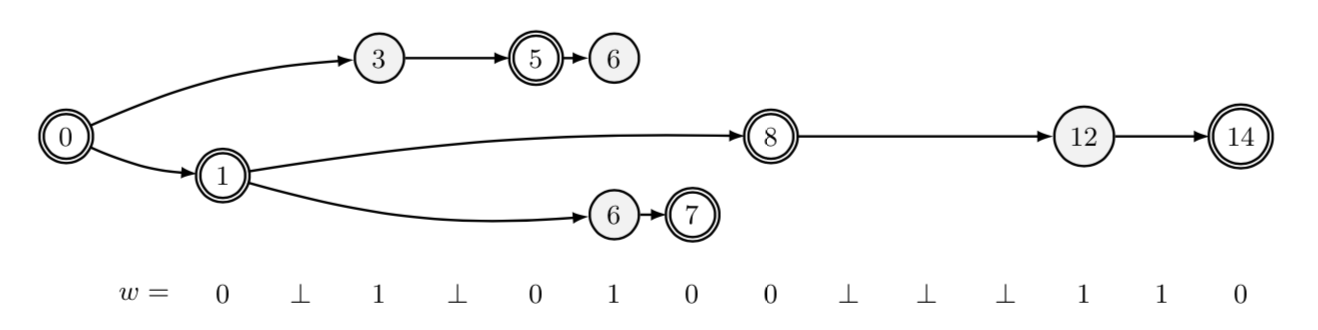
\includegraphics[width = \linewidth]{images/ouro-delta-fork.png}
    \caption{3-fork for characteristic string $w$}
    \label{fig:delta-fork}
\end{figure}

A fork contains tines which is covered in section \ref{sec:ouro-anal}, though an alteration to the viability of a tine is made to include the delay $\Delta$. For a tine to be viable with regard to $\Delta$, the inequality $lenght(t) \geq \max_{h+\Delta \geq \ell(t)} \textbf{d}(h)$, where $h$ is an uniquely honest index, should be true. Furthermore, tines can be measured by a quantity called \emph{divergence}, which is also covered in section \ref{sec:ouro-anal}, the only alteration to the definition of divergence is that the tines should be $\Delta$-viable. \\

%% Dominant distribution
Lastly, before showing the three properties; \emph{common prefix}, \emph{chain growth} and \emph{chain quality}, the distribution on characteristic strings will be formalized. The distribution is denoted $D_{\mathcal{Z}, A}^f$, where the distribution is determined by the the adversary, the environment and the parameter $f$. Here $f$ defines the relationship between the relative stake of a stakeholder and the probability that, the stakeholder will get elected as leader for a given slot. In \cite{ouroboros-praos}, a dominant distribution is defined in the following way.

\begin{mydef}[The dominant distribution $D^f_{\alpha}$]
\label{def:praos-dom-dist}
For two parameters $f$ and $\alpha$ define $D^f_{\alpha}$ to be the distribution on strings $w \in \{0,1,\perp\}^R$ that independently assigns each $w_i$ so that $p_{\perp} \overset{\Delta}{=} Pr[w_i = \perp] = 1 - f$, $p_0 \overset{\Delta}{=} Pr[w_i = 0] = \phi(\alpha) \cdot (1 - f)$, and $p_1 \overset{\Delta}{=} Pr[w_i = 1] = 1 - p_{\perp} - p_0$
\end{mydef}

The dominant distribution $D_{\alpha}^f$ is said to dominate the distribution $D_{\mathcal{Z},A}^f$, whenever there is a static adversary, who has relatively corrupted less than or equal to $1-\alpha$ share of the total stake. Since a distribution can dominate another distribution, their relation can be described by the partial order $\preceq$. For two distributions $D, D^{'}$, if $D \preceq D^{'}$, then $D^{'}$ is at least as adversarial as $D$, meaning that characteristic strings drawn from $D^{'}$ is at least as adversarial as the strings drawn from $D$. Thereby, a legal fork for a string from $D$ will also be a legal fork for a string from $D^{'}$. Furthermore, the divergence on the string drawn from $D$ will be less than or equal to the divergence on the string drawn from $D^{'}$.

\subsubsection*{Common Prefix, Chain Growth, and Chain Quality}
\label{subsec: praos-cpcgcq}

% Common Prefix
\begin{theorem}[Common prefix]
    Let $k,R,\delta \in \mathbb{N}$ and $\epsilon \in (0,1)$. Let $A$ be an $\alpha$-dominated adversary against the protocol $\pi_{SPoS}$ for some $\alpha$ satisfying $\alpha (1-f)^{\Delta} \geq (1+\epsilon)/2$. Then the probability that $A$, when executed in a $\Delta$-semisynchronous environment, makes $\pi_{SPoS}$ violate the common prefix property with parameter $k$ throughout a period of $R$ slots is no more than $e^{\ln R + \Delta - \Omega(k)}$. The constant hidden by the $\Omega(\cdot)$-notation depends on $\epsilon$.
\end{theorem}

% Proof
To prove the common prefix theorem, \cite{ouroboros-praos} shows that $\pi_{SPoS}$ violates the common prefix property with parameter $k$, when the event occurs that a $\Delta$-fork $F$ has $div_{\Delta}(F) \geq k$, and that this event should occur with probability no more than $e^{\ln R + \Delta - \Omega(k)}$. 

\begin{align*}
    Pr[div_{\Delta}(F) \geq k] &\leq Pr_{D^f_{\mathcal{Z},A}}[div_{\Delta}(w) \geq k]\\
                        &\leq Pr_{D_{\alpha}}[div_{\Delta}(w) \geq k]\\
                        &\leq e^{ln \; R - \Omega(k-\Delta)}
\end{align*}

The first inequality follows from the definition of $div_{\Delta}(w)$ which finds the largest $\Delta$-fork for $w$, and thereby $div_{\Delta}(F) \leq div_{\Delta}(w)$. The second inequality follows from the definition of $\alpha$-dominated adversaries, which states that $A$ is $\alpha$-dominated if the distribution $D^f_{\mathcal{Z},A}$ that upon the characteristic string $\{w\}$ satisfies $D^f_{\mathcal{Z},A} \preceq D^f_{\alpha}$. The last inequality follows from theorem 4 in \cite{ouroboros-praos} which states that; 



\emph{Given an \emph{active slot coefficient} $f \in (0,1], \Delta \geq 1$ and $\alpha$ s.t. $\alpha(1-f)^{\Delta} = (1+\epsilon)/2, \; \epsilon > 0$, and a characteristic string $w$ drawn from $w \in \{0,1, \perp\}^R$ according to $D^F_{\alpha}$. Then $Pr[div_{\Delta}(w) \geq k + \Delta] = 2^{-\Omega(k)+Log R}$}

% Chain Growth
\begin{theorem}[Chain growth]
    Let $k,R,\delta \in \mathbb{N}$ and $\epsilon \in (0,1)$. Let $A$ be an $\alpha$-dominated adversary against the protocol $\pi_{SPoS}$ for some $\alpha > 0$. Then the probability that $A$, when executed in a $\Delta$-semisynchronous environment, makes $\pi_{SPoS}$ violate the chain growth property with parameters $s \geq 4\Delta$ and $\tau = c\alpha/4$ throughout a period of $R$ slots, is no more than $exp(-c\alpha s/(20\Delta) + \ln R\Delta + O(1))$, where $c$ denotes the constant $c := c(f,\Delta) = f(1-f)^\Delta$. 
\end{theorem}

% Proof
To prove the chain growth theorem, \cite{ouroboros-praos} starts by defining an increasing sequence of slots $\hat{Sl}_1,\dots,\hat{Sl}_h$, which are $\Delta$-right-isolated slots and uniquely honest, namely $w_i = 0$. The notion of $\Delta$-right-isolated, means that the $\Delta$ slots after $w_i$ are $\perp$, i.e., empty. These slots are placed among the slots in the set $T = \{sl_1+\Delta, sl_1+\Delta+1, \dots, sl_2-\Delta\}$, and thereby will $\hat{sl}_1 \geq sl_1+\Delta$.

The leader of $\hat{sl}_1$ knows the chain $C_1$ and will therefore diffuse a chain at least as long as $C_1$, due to $C_1$ is being considered by the \emph{maxvalid} function, which leads to the chain being diffused by the leader will be at least $length(C_1)+1$ long. This progress continues for all the slots $sl_i$ for $i = 1,\ldots, h$. At the end at slot $sl_h$ the leader will diffuse a chain, that will be known to everyone at $sl_2$ and thereby, chain $C_2$ will be at least as long as this chain.

In order to bound the value $h$, it will be formalized to $H_T(x) = h$ for $x \xleftarrow{} D^f_{\mathcal{Z},A}$, where $x=\{0,1,\perp\}^R$ with respect to $T$. Furthermore, $H_T(x) \leq \tau s = c \alpha s /4$ is monotone and thereby it follows that $D^f_{\mathcal{Z},A} \preceq D_{\alpha}^f$ from the definition of $\alpha$-dominated adversaries, which implies
\begin{align*}
    \underset{x \xleftarrow{} D^f_{\mathcal{Z},A}}{Pr} [H_T(x) < c \alpha s / 4] \leq \underset{x \xleftarrow{} D^f_{\alpha}}{Pr} [H_T(x) < c \alpha s / 4]
\end{align*}


Consider $x \xleftarrow{} D^F_{\alpha}$, $\forall t \in T$ let $X_T$ denote a random variable which indicate whether or not $\hat{sl_1}$ is a $\Delta$-right-isolated uniquely honest slot. According to definition \ref{def:praos-dom-dist}
\begin{align}
    \mu = \mathbb{E}[X_t] = p_0p_{\perp}^{\Delta-1} \geq \alpha f(1-f)^{\Delta}
\end{align}
and furthermore, the random variables $X_t$ and $X_{t'}$ are independent if $|t-t'| \geq \Delta$

For a independent set of $X_t$, let $T_z = \{t\in T | t \equiv z \mod \Delta\}$ be used to index the independent $X_t$. Since $sl_2$ is at least $s\geq 4\Delta$ blocks ahead of $sl_1$, the size of the independent set is at least $|T_z| > \lfloor (s-2\Delta)/\Delta \rfloor \geq (s-3\Delta)/\Delta$. Thus it follows that


\begin{align*}
    Pr[\sum_{t \in T_z} X_t < \frac{\mu|T_z|}{2}] &\leq e^{-\frac{\mu|T_z| \delta^2}{2+\delta}}\\
    &= e^{-\frac{\mu|T_z|}{10}} \tag{Assuming that $\delta = \frac{1}{2}$} \\
    &\leq e^{-\frac{\mu|T_z|}{20}} \\
    &\leq e^{-\frac{\mu(s-3\Delta)}{20\Delta}}
\end{align*}

If it happens that $\Sigma_{t\in T_{z}} X_t \geq \mu |T_z|/2$ for each $z$, then $H_T(x) = \Sigma_{t\in T_{z}} X_t \geq \mu |T_z|/2 \geq \mu\hat{s}/2$, where $ \hat{s} \overset{\Delta}{=}s-2\Delta$. From the union bound it follows that:
\begin{align*}
    \underset{x \xleftarrow[]{} \mathcal{D}^f_{\alpha}}{Pr}[H_T(x) < \mu \hat{s} / 2] \leq \Delta \cdot e^{-\frac{\mu(s-3\Delta)}{20\Delta}}
\end{align*}

Since $\mu \geq \alpha f(1-f)^{\Delta}$ and $s \geq 4 \Delta$ it follows that $\hat{s} \geq \frac{s}{2}$
\begin{align*}
    \underset{x \xleftarrow[]{} \mathcal{D}^f_{\alpha}}{Pr} [H_T(x) < c \alpha s/4] = \Delta \cdot e^{-\frac{c \cdot \alpha(s-3\Delta)}{20\Delta}}
\end{align*}

Applying the union bound with $R$ slots in an epoch the probability that the chain growth property is violated with parameters $s$ and $\tau = c\alpha/4$.

\begin{equation*}
    R \cdot \Delta \cdot e^{\frac{-c\alpha(s-3\Delta)}{20\Delta}} = e^{-\frac{c\alpha(s-3\Delta)}{20\Delta} + ln R \Delta}
\end{equation*}

% Chain Quality
\begin{theorem}[Chain quality]
    Let $k,R,\delta \in \mathbb{N}$ and $\epsilon \in (0,1)$. Let $A$ be an $\alpha$-dominated adversary against the protocol $\pi_{SPoS}$ for some $\alpha > 0$ satisfying $\alpha(1-f)^{\Delta} \geq (1+\epsilon)/2$. Then the probability that $A$, when executed in a $\Delta$-semisynchronous environment, makes $\pi_{SPoS}$ violate the chain quality property with parameters $k$ and $\mu = 1/k$ throughout a period of $R$ slots, is no more than $e^{\ln R - \Omega(k)}$. 
\end{theorem}

The chain quality follows directly from lemma 4 in \cite{ouroboros-praos}, which states;

\begin{lemma}
Let $k, \Delta \in \mathbb{N}$ and $\epsilon \in (0,1)$. Let $A$ be an $alpha$-dominated adversary against the protocol of $\pi_SPoS$ for some $\alpha > 0$ satisfying $\alpha(1-f)^{\Delta} = (1+\epsilon)/2$. Let $B_1, \dots, B_k$ be a sequence of consecutive blocks in a chain $C$ possessed by an honest party. Then at least one block $B_i$ was created in a $\Delta$-right-isolated uniquely honest slot, except with probability $e^{-\Omega(k)}$.
\end{lemma}

For notation, slots are referred to as \emph{good} if it is $\Delta$-right-isolated and uniquely honest and \emph{bad} if it is neither empty nor good. Blocks are also respectively referred to as good or bad blocks.

For the proof assume all blocks $B_1,\dots,B_k$ are bad in order to show a contradiction. Let $G_1$ be the first good block preceding $B_1$ created in slot $\hat{sl}_1$ and $G_2$ be the first good block after $B_k$ created in slot $\hat{sl}_2$. Denote $T$ to be the sequence of slots between $\hat{sl}_1$ and $\hat{sl}_2$, excluding $\hat{sl}_1$ but including $\hat{sl}_2$. From the proof of chain growth it followed that in each good slot the chain would have its depth increase by at least 1 s.t. $\textbf{d}(G_2) \geq \textbf{d}(G_1) + g$, where g is the number of good slots in $T$. However since the chain consists of only bad slots, it follows that it increases with $\textbf{d}(G_2) \leq \textbf{d}(G_1) + b$. This can only be satisfied when $g \leq b$, in which it is only required to show that this is very unlikely to happen.

Let $E = \{x \in \{0,1,\perp\}^R | g(x) \leq b(x)\}$, where $g(x)$ is the number of good slots indexed by $T$ in $x$, while $b(x)$ being the bad slots indexed by $T$ in $x$. $E$ is monotone which means that $D^f_{\mathcal{Z},A} \preceq D^f_{\alpha}$ which implies
\begin{align}
    Pr_{D^f_{\mathcal{Z},A}}[g(x) \leq b(x)] \leq Pr_{D^f_{\alpha}}[g(x) \leq b(x)]
\end{align}
From the fact that $\alpha > 0$ and satisfies $\alpha(1-f)^{\Delta} = (1+e)/2$ and from lemma 3 in \cite{ouroboros-praos}, which notes that good slots are sampled with higher probability than bad ones, this results in $g(x) \leq b(x)$ for $x \xleftarrow{} D^f_{\alpha}$ falling exponentially in the size of $k$.

\subsubsection{Extension to a dynamic stake model}
Praos uses the same approach as Ouroboros to extend the static model to a dynamic model by dividing the execution of the protocol into epochs. This is first shown with a so-called \emph{leaky beacon} functionality, which is different as the adversary is allowed to make a number of resets of the randomness on this beacon, as well as knowing this randomness some blocks beforehand. The functionality is parameterized by two values $\tau$, which is how many slots prior to the end of a epoch the functionality leaks the randomness, and $r$ how many times the adversary is allowed to reset the randomness in the functionality. After an epoch has started no more resets are allowed to the functionality.\\

The protocol used to replace the randomness is to use the first $8k$ blocks of a $24k$ long periods resulting proofs for the random value, s.t., the next nonce $n_{j+1}$ is computed as $n_{j+1} = H(\eta_j || j+1 || y_1 || \dots || y_{8k})$. To show the security of this, \cite{ouroboros-praos} reduces the adversary of the basic properties of the blockchain to a resettable-beacon adversary. Such that the the adversary when able to get generate a block also have the posibility to "reset" the nonce, by having the choice of wanting to affect the next epochs nonce or not. Even in the case where the adversary has many potential resets, bounding the power of such an adversary is also taken into consideration. This is modeled by a random oracle as used in the analysis for Bitcoin in section \ref{subsec:anal-bitcoin}, where a adversary can make $q$ queries for hashing values. They conclude the hashing bound of the adversary to be $\approx 8qtk$, where $t$ is the amount of parties the adversary controls.


\section{Discussion}

% Both
%% Complex protocols comparatively
%% In depth analysis and proofs, peer reviewed IACR 2017 ouroboros; https://www.iacr.org/conferences/crypto2017/acceptedpapers.html
%% and eurocrypt 2018 praos https://eurocrypt.iacr.org/2018/acceptedpapers.html'
%% should still be noted that it was fairly recently the conference was held.
Both of the protocols covers a very in depth formulation of their protocols and using strong cryptographic foundations to show the security of their protocol. This is also reflected in being accepted papers in the International Association for Cryptologic Research \cite{iacr-ouro} \cite{iacr-praos}. Their formulation of abstracting the required cryptographic primitives into functionalities allows the focus to be on the protocol and its validity, while not having to worry about cryptographic primitives failing. Despite not having covered any of the possible implementations of the functionalities in our analysis, \cite{ouroboros} and \cite{ouroboros-praos} do propose possible implementations of the protocols.

Fully explaining the models as well as providing rigorous proofs for the protocols also involve some overhead in terms of complexity. It means many primitives have to be explained in detail to show security as well as having some insight into how security is shown for cryptographic protocols in general, such as the random oracle model used for hash functions as well as insights into the standard model. Though for obvious reasons having a complex well-defined model of computation is desired over having no model. 

% complexity, but is related to cryptographic proofs
In general the complexity of \cite{ouroboros} and \cite{ouroboros-praos} are more complex compared to Bitcoin. The Bitcoin protocol only uses two cryptographic primitives for the protocol; a public key signature infrastructure and a hash function, both of which are very common in practical applications.\\

% Our inputs - Ouroboros
%% All proposers are known beforehand, this creates the issue that an adversary can simple deny the proposer the ability to propose in his timeframe. E.g. DDOS propser such that they can never include a block within their timeframe
%% Required timing within the algorithm to propose and open random values - Guarantees completely random values
%% Already in use in the cardano cryptocurrency https://www.cardano.org/en/ouroboros - Does have the limitations that blocks have to be propagated in before creating new blocks as in Bitcoin - stated in the model, but implementaion is a lot faster 20 sec per block. - bernardo said so.
% More advanced cryptographic stuff. + synchrony
The Ouroboros protocol makes uses of a entirely new set of cryptographic primitives from multiparty computation, utilized in the Guaranteed Output Delivery coin tossing algorithm for providing randomness in the next epoch's genesis block. This requires honest parties to participate in the protocol in the designated time-frames set to make commitments, i.e., $4k$ for commit phase, $4k$ for reveal phase and $2k$ for recovery phase. This makes higher demands for synchrony for the honest peers throughout the execution of the protocol, and also when their designated time slot is to create blocks. Synchronizing clocks across multiple peers rarely posses a problem in practice, but it does complicate the implementation of the protocol. 

Ouroboros, despite the complexity of the G.O.D. coin flipping protocol, does have the advantage of having perfect randomness generation for each epoch, which in turn also creates a perfectly random leader selection, for each epoch.\\

The Ouroboros protocol is currently utilized as the core protocol in the Cardano cryptocurrency \cite{cardano-ouro}, which is currently ranked 8th cryptocurrency in terms of market cap. Despite being limited that the network needs to synchronize as in Bitcoin, the speed of which blocks are created is much faster compared to that of Bitcoin. After a brief and informal discussion with Bernardo David, the block creation time is around 20 seconds, but is a tweakable parameter in the system to guarantee network synchronization.

An attack vector that can become an issue in a concrete instantiation of the protocol, is that the slot leader election is deterministic, and all known public keys of the stakeholders are known. If an adversary is able to disclose the identity of the owner of the given honest blocks, he can execute a Denial-of-Service attack, letting the adversary have more influence on the blocks created. In the described model, this is covered by always assuming that at least $50\%$ of the slot leaders are active. As such a small remark that the protocol has to provide some privacy guarantees is made. Privacy of the protocol is not covered in this thesis, but Ouroboros does also mention privacy guarantees in \cite{ouroboros}. \\


% Praos
%% Multiple people can propose blocks in a single time slot / or none
%% Person is hidden behind the Hash function
%% Nonce for leader selection is found from how the protocol executes, but that means that an adversary can influence it - Efficient
% KES and VRF is new sexy crypto stuff + synchrony
The Praos protocol, requires synchrony to a lesser extent with only having requirements of when peers need to generate new blocks. While Praos also makes use of primitives that are not as common, such as key evolving signatures and verifiable random functions, for the protocol to be executed. This does minimize communication to a certain extent, not having to include shares as in Ouroboros throughout the execution of the protocol.

The Praos protocol does guarantee some additional security properties compared to that of the Ouroboros protocol. First off the block proposers are, unlike the Ouroboros protocol, not known until the time when it is the peers turn, as the proposer is hidden in the verifiable random function. As such unless an adversary can compromise the secret key of the verifiable random function, then the adversary cannot identify which stakeholder is going to generate a block for the given slot. This creates a neat innate privacy when generating blocks, though of course the identity of the stakeholder is known when the block is published. Praos also has a less rigid slot leader selection scheme, it is a probabilistic proposal system, such that the leader selection algorithm is not guaranteed to be only a single stakeholder. A slot can be assigned to no stakeholders, or in unlikely cases assigned to more than a single stakeholder. Thus making the chain not grow, the chain growth theorem does show that this only happens with negligible probability, or creating forks, which common prefix and common prefix guarantees only happens with negligible probability.

Praos also have extended security guarantees by capturing the delay of messages with the $\mathcal{F}_{DDiffuse_{\Delta}}$ functionality, allowing an adversary to delay messages to honest peers by a certain $\Delta$. As given a real network, such delays can occur, given adversarial influence or not, as such given the extension to this in the functionality is a great addition. The model also assumes instant corruption over a delayed corruption the Ouroboros protocol, which provides a stronger security guarantee.


These additional security guarantees do not come without a cost though. The randomness generated for each epoch is not entirely random as in Ouroboros, which is reflected in the leaky resettable randomness beacon. As an adversary can choose to include a block or not, he can affect the randomness of the next epoch, thus selecting the randomness that better suits him for the next epoch. The model they describe, where the adversary is freely able to reset the beacon when he chooses before the next epoch starts, is a more powerful model compared to the one he, in reality, would have. In reality, the adversary only has the ability to select to include a block or not. Intuitively, assuming a perfect hash function, when an honest party includes a block, the result of the hash function would be perfectly random. As such having done resets prior to this i.e., included blocks or not, would simply be a gamble on the total randomness of the honest block. Meaning only if the adversary has the last $x$ blocks of $8k$ blocks that determine the randomness, would be able to see the final randomness and thus choosing which results suit him best.\\


%% Comparison of the chain quality - chain growth and common prefix, also include PoW just in comparison
Both \cite{ouroboros} and \cite{ouroboros-praos} show that an adversary can make their protocols violate the \emph{common prefix}, \emph{chain growth} and \emph{chain quality} properties with an exponentially decreasing probability based on their presented security models.\\


It should be noted that this thesis has only covered two chain-based PoS protocols, which were heavily selected based on their insights into how to model such a blockchain system, and provide security guarantees. Many protocols do not go as in-depth into showing the security, while only providing security against a set of attack vectors and concluding that the protocol is secure. As such future work could include analysis into other Proof-of-Stake approaches, such as Algorand \cite{algorand}, which instead relies on $2/3$ honest parties and is a Byzantine fault tolerance based PoS protocol, could be very interesting. 